\part{Introdution : généralités et contexte} % (fold)
\label{prt:introduction_ _théorique_}
	
	\section{BCI} % (fold)
	\label{sec:intro_bci}
	
	BCI: Brain Computer Interface (ou Interface Cerveau-Machine en français).
	Aussi appelée Interface Neuronale Directe (abrégée IND), il s'agit d'une interface de communication directe entre un cerveau et un composant externe (généralement un ordinateur).

	
	\section{EEG} % (fold)
	\label{sec:eeg}
	\begin{figure}[h!]
			\centering
		    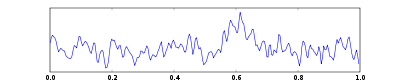
\includegraphics []{figures/eeg_1s_signal.png} \\
		    \captionof{figure}{ci-dessus une seconde de signal EEG}
			\label{fig_eeg_1s}
	\end{figure}
	EEG ou électroencéphalographie est une technique de mesure de l'activité électrique du cerveau mesurée à l'aide d'électrodes placées sur le cuir chevelu. L'EEG est un examen indolore est non-invasif comparativement à l'iEEG(électroencéphalographie intracrânienne) qui, elle, place les électrodes sous la surface du crâne. le signal EEG obtenu est la résultante de la sommation d'un potentiel d'action post-synaptique synchrone issu d'un grand nombre de neurones.
	\begin{figure}
		\centering 
	 	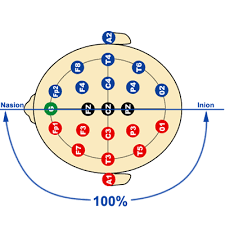
\includegraphics [width=7cm,height=7cm]{figures/captoreeg.png} \\
		\captionof{figure}{position des capteurs}
		\label{fig_captors}	
	\end{figure}

	% section eeg (end)
	
	% section bci (end)

	\section{Généralités} % (fold)
	\label{sec:généralité}
	
	Ici, certains concepts clés doivent être définis pour comprendre en quoi consiste notre projet: 
	\subsection{Les réseaux de neurones} % (fold)
	\label{sub:les_réseaux_de_neurones}
	 Les réseaux de neurones sont un modèle de calcul représentant schématiquement les réseaux de neurones biologiques. C'est à celui-ci que 
	l'on va imposer l'apprentissage d'un échantillon de données. Pour cela, nous allons 
	utiliser l'algorithme du gradient, le gradient étant, en mathématiques, un vecteur qui
	 représente la variation d'une fonction en fonction de la variation de ses paramètres. Tout
	  comme nous, le réseau de neurones n'est pas parfait et fera des erreurs lors de son 
	  apprentissage. Il faudra donc utiliser la rétro-propagation du gradient qui est un algorithme 
	  servant à corriger les erreurs du réseau de neurones pour qu'il ne les reproduise pas.
	% subsection les_réseaux_de_neurones (end)

	\subsection{Notions en lien avec BCI} % (fold)
	\label{sub:notion_lien}
	Certaines notions sont importantes à connaître lorsque l'on s’intéresse au BCI, entre autres le SSVEP  et le P300. Ce sont tous les deux des réponses naturelles à une stimulation visuelle. Pour le SSVEP, la réponse est détectée lors d'une stimulation visuelle lorsque la rétine est excitée par un stimulus visuel dont la fréquence d'affichage est entre 3.5Hz et 75Hz. Le P300, par contre, 
	est une réponse qui apparaît 300ms après stimulation visuelle. 
	% subsection interface_type_ssvep (end)
	
	% section généralité (end)

	\section{Contexte} % (fold)
	\label{sec:contexte}
	
	   Les réseaux de neurones sont des composants logiciels informatiques permettant de représenter de manière aproximative les réseaux de nehruones humains.

       Ceux-ci permettent, via une méthode d'apprentissage basée sur le gradient d'erreur que l'on modifie jusqu'à ce que la réponse donnée par le réseau de neurones soit la bonne.

	   Dans le cadre de ce projet, nous devions développer un réseau de neurones afin de contrôler automatiquement les activités cérébrales d'un sujet. Ainsi, le système pourrait nous dire grâce au signal EEG du patient quelle activité il est en train de faire ou bien quel est son état. Notre système pourrait donc par exemple connaître l'activité d'un malade d'Alzheimer telle que :
	   \begin{itemize}
	   	\item[-] la lecture;
		\item[-] l'attention sur un film;
		\item[-] l'écriture;
		\item[-] la discussion;
		\item[-] le repos.
	   \end{itemize}

	   Ceci est un exemple d'utilisation de ces réseaux de neurones. Or, il se trouve que nous pouvons les utiliser pour des choses plus sofistiquées telles que :
	   \begin{itemize}
	   \item[-]la détermination de facteurs dominants dans le déclanchement d'une maladie afin de mieux la comprendre et de cibler la recherche afin d'essayer de trouver un traitement.
	   \item[-]l'amélioration de la qualité de vie de personnes lourdement handicapées: traitement des signaux représentant les pensées de la personne pour qu'elle puisse bouger ses bras ou communiquer (si elle ne le peut pas verbalement)
	   \item[-]dans notre cas, peut-être que ce projet permettrait de davantage retarder l'évolution de la maladie d'Alzheimer en essayant de stimuler la pensée des patients afin qu'ils puissent conserver leur autonomie un maximum par le procédé du traitement du signal.
	   \end{itemize}
	
	
	
	
		% Contexte et Problématique 
	% section contexte (end)

% part introduction_ _théorique_ (end)